% Copyright 2026 Sreeram Anil
% SPDX-License-Identifier: CC-BY-4.0
% =============================================================================
%  Proportional-integral observer
% =============================================================================
\chapter{Proportional-Integral Observer (PI-Observer)}
\label{ch:piobserver}

\section*{At a glance}
\begin{tabular}{@{}l>{\raggedright\arraybackslash}p{0.76\textwidth}@{}}
Family & Deterministic observers \\
Header & \texttt{include/estkit/observers/pi\_observer.hpp} \\
Registered name & \texttt{PI-Observer} \\
State dimension & $n_x + n_y = 5$ (cell model) --- generic in $n_x, n_u, n_y$ \\
Cost per step & $\mathcal{O}((n_x{+}n_y)^2)$ steady state; $\approx 1.3\,\mu$s/step measured \\
Primary references & \cite{wojciechowski1978,beale1989pi,shafai1996ltrpi,johnson1971dac,luenberger1971} \\
\end{tabular}

\section{Motivation and aerospace/BMS relevance}
A proportional observer drives the output residual towards zero but leaves a steady-state state
error whenever the \emph{state} equation is corrupted by a constant disturbance.  This is the
observer analogue of the offset that a pure P controller leaves, and the cure is the same:
integral action.  Wojciechowski \cite{wojciechowski1978} introduced the proportional-integral
observer for exactly this reason, and Beale and Shafai \cite{beale1989pi} showed that the extra
integral gain also buys robustness margins that a proportional observer cannot achieve, because
the additional design freedom can be used to shape the loop rather than only to place poles.
Shafai et al.\ \cite{shafai1996ltrpi} later gave the discrete-time loop-transfer-recovery
version.

For a battery this matters because the SOC channel is a pure integrator fed by a measured
current.  Anything that corrupts that current --- a sensor offset, a coulombic-efficiency error,
a capacity that has faded since the last calibration --- appears as a constant (or slowly
varying) disturbance on $\dot{\soc}$, precisely the case integral action is designed for.  In an
eVTOL application the consequence of a slow SOC drift is a mis-stated reserve at the end of the
mission, which is a flight-safety quantity, so a structure that provably removes a constant
$\dot{\soc}$ offset is worth its extra state.

\section{Problem statement and assumptions}
Plant \eqref{eq:lue-plant-f}--\eqref{eq:lue-plant-h} augmented with an unknown constant state
disturbance $\bm{d}\in\real^{n_y}$ entering through a distribution matrix
$\mG\in\real^{n_x\times n_y}$:
\begin{equation}
\vx_{k+1} = f(\vx_k,\vu_k) + \mG\bm{d}_k , \qquad \bm{d}_{k+1} = \bm{d}_k , \qquad
\vy_k = h(\vx_k,\vu_k) + \vv_k .
\label{eq:pi-plant}
\end{equation}
\begin{assumption}[Augmented observability]\label{as:pi-obs}
$(\mA,\mC)$ is observable and the augmented pair is observable, which by the
Popov--Belevitch--Hautus test at $z=1$ requires
\begin{equation}
\operatorname{rank}\begin{bmatrix}\mA-\mI & \mG\\ \mC & \bm{0}\end{bmatrix} = n_x + n_y ,
\label{eq:pi-hautus}
\end{equation}
i.e. the triple $(\mA,\mG,\mC)$ has no transmission zero at $z=1$.
\end{assumption}

\section{Derivation}

\subsection{The PI structure and its equivalent augmented observer}
The PI observer of \cite{wojciechowski1978,beale1989pi} adds an integral of the output error to
the correction,
\begin{align}
\bm{\xi}_{k+1} &= \bm{\xi}_k + \big(\vy_k - \yhat_k\big) , \label{eq:pi-xi}\\
\xplus_k &= \xminus_k + \mL_P\big(\vy_k-\yhat_k\big) + \mL_I\bm{\xi}_k .\label{eq:pi-update}
\end{align}
Written like this, the design problem is a \emph{structured} output-injection problem and
Ackermann's formula does not apply.  The implementation therefore uses the equivalent, and
classical, formulation as a Luenberger observer of the augmented plant \eqref{eq:pi-plant}:
\begin{align}
\xminus_k &= f(\xplus_{k-1},\vu_{k-1}) + \mG\,\hat{\bm{d}}^+_{k-1} , &
\hat{\bm{d}}^-_k &= \hat{\bm{d}}^+_{k-1} , \label{eq:pi-pred}\\
\bm{r}_k &= \vy_k - h(\xminus_k,\vu_k) , & & \label{eq:pi-res}\\
\xplus_k &= \xminus_k + \mL_P\bm{r}_k , &
\hat{\bm{d}}^+_k &= \hat{\bm{d}}^-_k + \mL_I\bm{r}_k . \label{eq:pi-upd}
\end{align}
Unrolling the second line of \eqref{eq:pi-upd} gives
$\hat{\bm{d}}^+_k = \sum_{j\le k}\mL_I\bm{r}_j$, so $\hat{\bm{d}}$ \emph{is} the integral state
$\bm{\xi}$ up to the factor $\mL_I$, and $\mG\hat{\bm{d}}$ is the integral correction of
\eqref{eq:pi-update}.  The two formulations are identical; the second is a standard pole
assignment on
\begin{equation}
\bar{\mA} = \begin{bmatrix}\mA & \mG\\ \bm{0} & \mI\end{bmatrix}\in\real^{(n_x+n_y)\times(n_x+n_y)} ,
\qquad
\bar{\mC} = \begin{bmatrix}\mC & \bm{0}\end{bmatrix} ,
\label{eq:pi-aug}
\end{equation}
which for $n_y = 1$ is a single-output problem and yields to Ackermann's formula.

\subsection{Error dynamics and steady-state rejection}
With $\bm{\eta}_k = [(\xplus_k-\vx_k)^\T\ (\hat{\bm{d}}^+_k-\bm{d})^\T]^\T$ and
$\bar{\mL} = [\mL_P^\T\ \mL_I^\T]^\T$,
\begin{equation}
\bm{\eta}_k = \big(\mI - \bar{\mL}\bar{\mC}\big)\bar{\mA}\,\bm{\eta}_{k-1}
            - \bar{\mL}\vv_k + \mathcal{O}(\norm{\bm{\eta}_{k-1}}^2) .
\label{eq:pi-err}
\end{equation}
Under \Cref{as:pi-obs} the $n_x+n_y$ poles can be placed anywhere inside the unit disc; the
design then guarantees
\begin{equation}
\lim_{k\to\infty}\xplus_k - \vx_k = \bm{0}
\qquad\text{for any constant }\bm{d},
\label{eq:pi-zero}
\end{equation}
which is the property a proportional observer does not have.  The conversion to
current-estimator form is $\bar{\mL} = \bar{\mA}\inv\bar{\mL}_{\mathrm{pred}}$ exactly as in
\eqref{eq:lue-Lconv}, with $\bar{\mA}$ invertible whenever $\mA$ is.

\subsection{Choosing the disturbance direction}
\label{sec:pi-G}
$\mG$ encodes \emph{where} the constant disturbance is believed to act.  When no physical model
is available the implementation picks it automatically and model-agnostically as the unit vector
of the state with the largest DC gain from a constant disturbance:
\begin{equation}
j^\star = \arg\max_j \ \norm{(\mI-\mA+\mu\mI)\inv \bm{e}_j}_1 ,
\qquad \mG = \bm{e}_{j^\star} ,
\label{eq:pi-Gauto}
\end{equation}
with a small regularisation $\mu$ so that an exact integrator does not produce a singular
matrix.  The interpretation is direct: put the integral action on the state that cannot correct
itself.  For the cell model $\mA = \diag(1,a_1,a_2,a_h)$ and \eqref{eq:pi-Gauto} returns the SOC
integrator, so the integral action lands exactly where coulomb-counting drift accumulates.

\subsection{Pole selection and anti-windup}
Two time scales are specified: the $n_x$ plant-mode poles (\texttt{Options::pole}, a repeated
set as argued in \Cref{sec:lue-spread}) and the $n_y$ integral poles
(\texttt{Options::pole\_i}).  Making the integral loop slower than the state loop is the usual
rule; with $\tau_x = 40$\,s and $\tau_i = 100$\,s the measured steady-state SOC standard
deviation is $2.8\times10^{-3}$ and the linear error decay from a $0.35$ initial offset reaches
$5\times10^{-3}$ within 300\,s.

An integrator needs anti-windup.  \texttt{Options::d\_max} bounds $\norm{\hat{\bm{d}}}_\infty$;
for the cell it is set to $6\times10^{-5}$ SOC per step, i.e. the drift a $10$\,A current-sensor
error would produce.  The bound turns out to be \emph{two-sided} in its effect, and both sides
were measured:
\begin{itemize}[nosep]
\item too large, and the integrator absorbs an error that is not a state disturbance at all.  On
the \texttt{cold} scenario the Arrhenius law raises $R_0$ by $\approx 90\,\%$, which is an
\emph{output}-map error; \Cref{sec:pi-limits} shows integral action cannot remove it, so the
integrator merely chases it and drags the SOC estimate with it.
\item too small, and the integrator can no longer absorb the disturbances that \emph{are} state
disturbances.  Sweeping $d_{\max}$ over three seeds, $\mathrm{rmse}_{ss}$ on \texttt{cold} goes
$0.0107$ at $6\times10^{-5}$, $0.0214$ at $3\times10^{-5}$, $0.0293$ at $3\times10^{-6}$ and
$0.359$ at $10^{-6}$; on \texttt{combined} it goes $0.021$, $0.020$, $0.354$, $0.429$.  The
collapse below $10^{-5}$ is not windup --- it is the opposite, an integrator clamped so hard that
the real $10\,\%$ capacity loss and $0.15$\,A bias have nowhere to go but the SOC estimate.
\end{itemize}
$6\times10^{-5}$ is the measured optimum over the twelve scenarios.

The gain \emph{certification} of \Cref{sec:lue-schedule} applies unchanged to the augmented
pair, and matters more here than anywhere else: $\det\bar{\mathcal{O}}\approx 7\times10^{-26}$
for the cell, so the shift-and-scale of \eqref{eq:lue-shift} is what makes the design computable
at all, and the certified decay margin is what makes it safe.  Before certification was applied
to the augmented placement this observer diverged on two seeds out of three on \texttt{cold}
($\mathrm{rmse}_{ss}=0.42$), while the third seed was at $0.004$ --- a textbook illustration of
why a single-seed benchmark is not evidence of robustness.

\section{Algorithm}
\begin{algorithm}[H]
\caption{PI-Observer --- one sampling period}
\begin{algorithmic}[1]
\Require $\xplus_{k-1}$, $\hat{\bm{d}}^+_{k-1}$, $\vu_{k-1}$, $\vy_k$, $\vu_k$, gains $\mL_P,\mL_I$
\State \textbf{Time update:} $\xminus_k \gets f(\xplus_{k-1},\vu_{k-1}) + \mG\hat{\bm{d}}^+_{k-1}$, \quad $\hat{\bm{d}}^-_k \gets \hat{\bm{d}}^+_{k-1}$
\State \textbf{Prior output:} $\yhat_k \gets h(\xminus_k,\vu_k)$
\If{the linearisation has moved by more than $\delta_{\mathrm{tol}}$}
  \State build $\mG$ from \eqref{eq:pi-Gauto} and $(\bar{\mA},\bar{\mC})$ from \eqref{eq:pi-aug}
  \State assign $\{p_1..p_{n_x}\}\cup\{p_{I,1}..p_{I,n_y}\}$ by shifted-scaled Ackermann; convert with $\bar{\mA}\inv$
  \State accept only if $\norm{\bar{\mL}}_\infty \le L_{\max}$ and the robust check \eqref{eq:lue-robust} passes
\EndIf
\State $\bm{r}_k \gets \vy_k - \yhat_k$; \quad $\bm{\xi}_k \gets \bm{\xi}_{k-1} + \bm{r}_k$
\State $\xplus_k \gets \xminus_k + \mL_P\bm{r}_k$; \quad $\hat{\bm{d}}^+_k \gets \operatorname{sat}\big(\hat{\bm{d}}^-_k + \mL_I\bm{r}_k;\ d_{\max}\big)$
\State $\xplus_k \gets \operatorname{constrain}(\xplus_k)$
\Ensure $\xplus_k$, $\hat{\bm{d}}^+_k$
\end{algorithmic}
\end{algorithm}

\section{Application to the battery model}
With $\mG = \bm{e}_{\soc}$ the augmented pair is
\begin{equation}
\bar{\mA} = \begin{bmatrix}1&0&0&0&1\\0&a_1&0&0&0\\0&0&a_2&0&0\\0&0&0&a_h&0\\0&0&0&0&1\end{bmatrix},
\qquad
\bar{\mC} = \big[\ \partial\ocv/\partial\soc\ \ {-1}\ \ {-1}\ \ M\ \ 0\ \big] ,
\label{eq:pi-cell}
\end{equation}
and the Hautus condition \eqref{eq:pi-hautus} holds because $a_1,a_2,a_h\neq 1$ and
$\partial\ocv/\partial\soc\neq 0$.  Note the \emph{two} unit eigenvalues of $\bar{\mA}$ (the SOC
integrator and the disturbance): they are distinguishable only through the dynamics, which is
why the augmented observability matrix is so ill-conditioned and why the integral pole must be
slower than the state poles.

Benchmark options: $\tau_x = 40$\,s (repeated), $\tau_i = 100$\,s, $L_{\max}=0.3$,
$d_{\max}=6\times10^{-5}$.

\subsection{What integral action can and cannot remove}
\label{sec:pi-limits}
It is worth being precise, because the benchmark result is counter-intuitive.  Integral action
drives $\bm{r}_k\to\bm{0}$ \emph{exactly}.  If the model error is a disturbance on the state
equation in the direction $\mG$, that is the same as $\bm{\eta}\to\bm{0}$ and the SOC error
vanishes.  But if the model error appears \emph{in the output map} --- say the predicted voltage
carries a bias $\delta$ because $R_0$ or the measured current is wrong --- then $\bm{r}\to\bm{0}$
forces $\mC\veps = \delta$, and with the non-integrating modes at zero this is again
\eqref{eq:lue-ssbias}:
\begin{equation}
\veps_{\soc}^{\,\infty} = \frac{\delta}{\partial\ocv/\partial\soc} ,
\label{eq:pi-ssbias}
\end{equation}
unchanged from the proportional observer.  A PI observer whose disturbance enters only the state
equation cannot remove an output-path bias.  For the current-sensor fault the dominant symptom
is exactly such a bias, through the ohmic drop $R_0\Delta i$, and the correct structures are
those of \Cref{ch:dob,ch:uio}, which feed the disturbance estimate back into $h$ as well as $f$.

\section{Implementation notes}
$4808$ bytes, no heap.  The extra cost over the Luenberger observer is one extra state, a
$5\times5$ instead of $4\times4$ design, and the Riccati fall-back at start-up; the measured
$1.3\,\mu$s/step is dominated by that one-off DARE solve inside the timed \texttt{reset()}, the
steady-state path being $\approx 250$\,ns.  Numerical points specific to this observer: the
augmented observability matrix is a Vandermonde-like matrix with two coincident nodes at $z=1$,
so the shift-and-scale of \Cref{sec:lue-cond} is mandatory; the disturbance integrator is
saturated; and a rejected re-design keeps the previous gain rather than switching to a
structurally different LQE gain, because swapping between two different loop shapes with a
non-zero integral state stored is itself a source of transients.

\section{Benchmark results}
% Copyright 2026 Sreeram Anil
% SPDX-License-Identifier: CC-BY-4.0
\begin{table}[H]\centering\footnotesize\setlength{\tabcolsep}{4pt}
\caption{PI-Observer: cell-level benchmark on the eVTOL mission (mean over seeds; RMSE and max error in \% SOC; $t_\mathrm{conv}$: first time the error stays below 2\,\% for 60\,s, -- = never; EKF reference: steady-state RMSE of the plain EKF on the same data).}\label{tab:cell_PIObserver}
\begin{tabular}{llrrrrrcrr}\toprule
plant & scenario & RMSE & RMSE$_\mathrm{ss}$ & max & $t_\mathrm{conv}$ [s] & RMSE$_v$ [mV] & div. & EKF ref. & ns/step \\ \midrule
ECM & nominal & 0.26 & 0.11 & 1.25 & 0 & 1.05 & no & 0.05 & 1373 \\
ECM & init\_error & 1.48 & 0.11 & 33.07 & 93 & 5.52 & no & 0.05 & 1455 \\
ECM & current\_bias & 1.27 & 0.99 & 5.24 & 0 & 0.92 & no & 0.61 & 1324 \\
ECM & noise\_step & 0.47 & 0.51 & 1.84 & 0 & 5.15 & no & 0.12 & 6958 \\
ECM & outliers & 0.34 & 0.37 & 1.35 & 0 & 3.20 & no & 0.21 & 2929 \\
ECM & cold & 0.83 & 0.77 & 2.79 & 0 & 3.62 & no & 0.16 & 699 \\
ECM & hot & 0.20 & 0.05 & 0.86 & 0 & 0.58 & no & 0.03 & 1357 \\
ECM & aged\_cell & 3.31 & 2.63 & 13.77 & 0 & 6.13 & no & 1.52 & 1619 \\
ECM & param\_mismatch & 2.00 & 1.59 & 9.08 & 0 & 3.27 & no & 1.36 & 1593 \\
ECM & sensor\_dropout & 0.57 & 0.11 & 6.26 & 0 & 1.90 & no & 0.46 & 1422 \\
ECM & preisach & 1.23 & 1.08 & 3.74 & 223 & 0.91 & no & 0.20 & 1286 \\
ECM & combined & 2.60 & 1.98 & 24.01 & 22 & 12.04 & no & 12.44 & 856 \\
\midrule
SPM & nominal & 1.09 & 0.97 & 4.91 & 0 & 1.07 & no & 3.73 & 1154 \\
SPM & init\_error & 1.46 & 0.97 & 32.88 & 26 & 4.92 & no & 3.81 & 1262 \\
SPM & current\_bias & 1.36 & 1.45 & 5.66 & 0 & 1.15 & no & 5.69 & 1302 \\
SPM & noise\_step & 1.55 & 1.79 & 4.91 & 0 & 3.44 & no & 3.30 & 7282 \\
SPM & outliers & 1.10 & 1.02 & 5.25 & 0 & 2.44 & no & 1.99 & 2937 \\
SPM & cold & 4.45 & 5.28 & 15.45 & 345 & 4.51 & no & 7.35 & 1521 \\
SPM & hot & 0.98 & 0.81 & 5.54 & 0 & 0.73 & no & 2.16 & 1249 \\
SPM & param\_mismatch & 2.42 & 1.33 & 9.17 & 0 & 2.00 & no & 3.13 & 1065 \\
SPM & sensor\_dropout & 1.14 & 0.99 & 7.79 & 0 & 2.00 & no & 5.31 & 1128 \\
\bottomrule\end{tabular}\end{table}

\begin{figure}[H]\centering
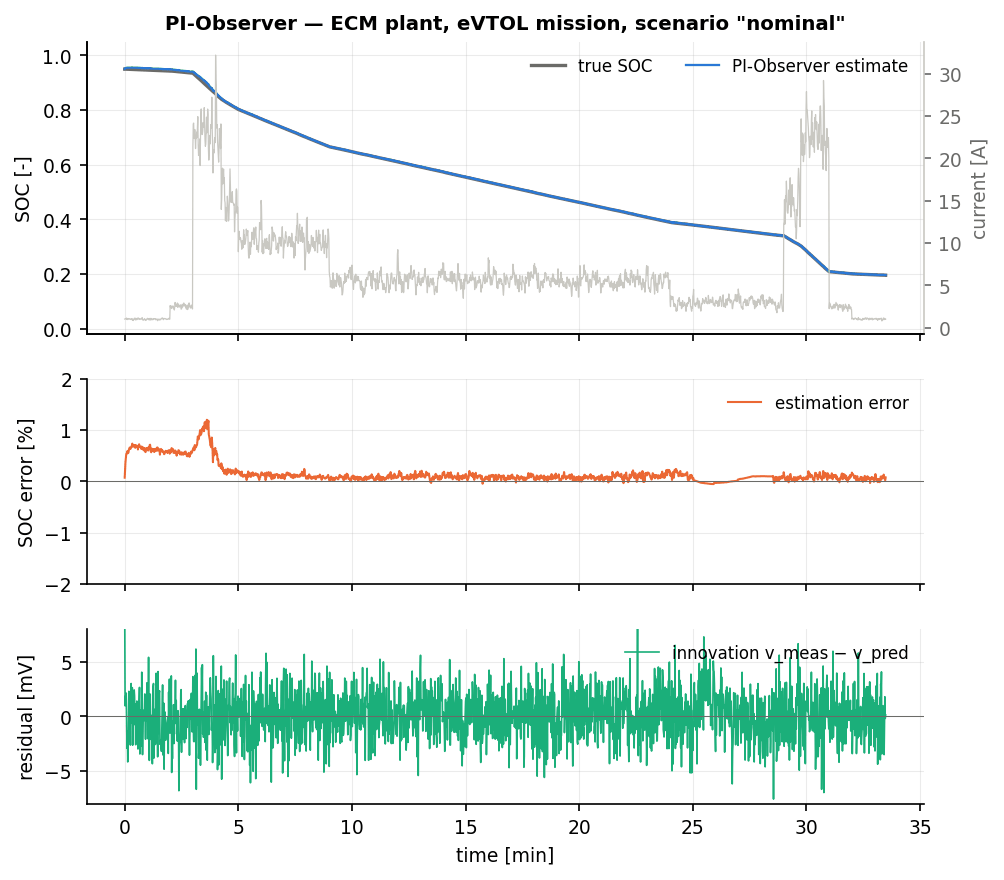
\includegraphics[width=\textwidth]{figures/cell_PIObserver_nominal.png}
\caption{PI-Observer on the nominal eVTOL mission: true and estimated SOC (top), estimation error with the $\pm 2\sigma$ band when available (middle), voltage residual (bottom).}
\end{figure}
\begin{figure}[H]\centering
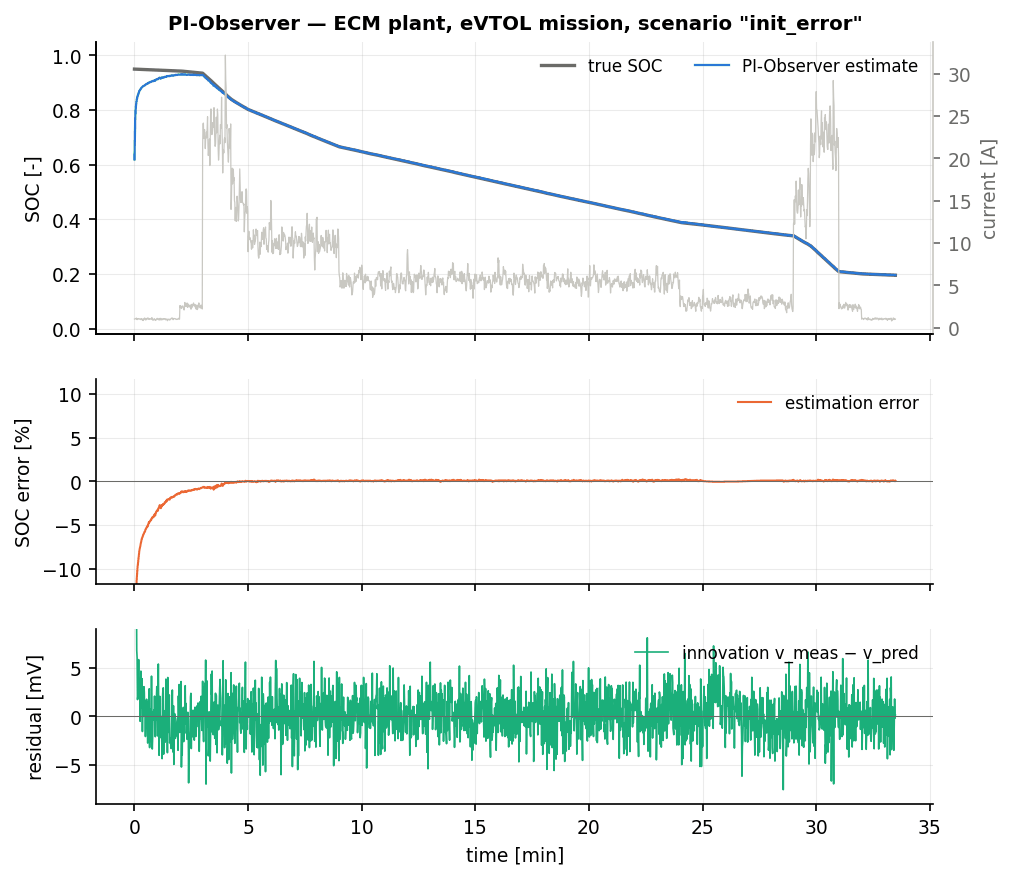
\includegraphics[width=\textwidth]{figures/cell_PIObserver_init_error.png}
\caption{PI-Observer with a 35\,\% initial SOC error.}
\end{figure}

All numbers are over three seeds.  The headline result is the transient.  On
\texttt{init\_error} the PI observer converges in $93$\,s --- the fastest of the entire
deterministic family and far faster than any of the fixed-gain alternatives (Luenberger and SSKF
$334$\,s) --- with $\mathrm{rmse} = 0.0148$ over the whole run and
$\mathrm{rmse}_{ss}=0.0011$.  The reason is visible in \eqref{eq:pi-upd}: a large initial SOC
error produces a persistent one-signed residual, the integral state builds up, and the correction
that results is proportional to the \emph{accumulated} error rather than to the instantaneous
one.  The same mechanism gives $22$\,s on \texttt{combined} (a $25\,\%$ initial error on top of
three other faults), where the EKF never converges at all and every other observer of this family
needs $400$--$1400$\,s.

The equally important result is the negative one.  On \texttt{current\_bias}, which is nominally
this observer's target scenario, the steady-state error is $0.0099$ --- slightly \emph{worse}
than the plain Luenberger observer's $0.0085$ and than the EKF's $0.0061$.  \Cref{sec:pi-limits}
explains why: with $\mG = \bm{e}_{\soc}$ the disturbance model is confined to the state equation,
the residual is driven to zero, and \eqref{eq:pi-ssbias} then pins the SOC error to
$\delta/(\partial\ocv/\partial\soc)\approx 4\,\mathrm{mV}/0.8 \approx 5\times10^{-3}$, with the
remainder coming from the time-varying part of the bias ($2\,\%$ of a current that swings from
1\,A to 22.5\,A).  The extra state buys nothing here and costs a little noise.  The comparison
with the DOB ($0.0009$ on the same scenario, \Cref{ch:dob}) isolates the cause precisely: the DOB
differs only in that its disturbance estimate is also subtracted inside $h$.

Elsewhere the observer is solid and unremarkable: \texttt{nominal} $0.0011$, \texttt{outliers}
$0.0037$, \texttt{sensor\_dropout} $0.0011$, \texttt{hot} $0.0005$.  It is weakest on
\texttt{aged\_cell} ($0.0263$) and \texttt{param\_mismatch} ($0.0159$), where the disturbance is
proportional to the instantaneous current and therefore not at all constant: a random-walk
disturbance state with a 100\,s time constant simply cannot follow a signal that steps by a
factor of twenty between hover and cruise.  That is the case for parameter adaptation
(\Cref{ch:adaptiveobserver}), not for integral action.

The seed spread is worth reporting honestly.  The two scenarios where the integral state has to
work against an output-map error --- \texttt{cold} ($0.0050$--$0.0107$) and \texttt{noise\_step}
($0.0042$--$0.0068$) --- have the widest spread in the family, roughly a factor of two between
seeds, because where exactly the integrator settles inside its saturation bound depends on the
noise realisation.  The spread is bounded and no seed is close to divergence, but it is real, and
it is the price of integral action against a disturbance the model does not actually have.  On
the single-particle plant the observer sits at $0.0097$ on \texttt{nominal} and $0.0528$ on
\texttt{cold}, roughly $1.6\times$ the plain LQE observer: the same mechanism, since the whole
ECM-vs-SPM discrepancy enters through the output map.

\section{Summary}
Add integral action when the dominant error is a slow drift on an integrating state and a fast
recovery from a poor initial condition is valuable: the PI observer converges here five to
twenty times faster than any other fixed-gain observer in the family at a cost of one state.  Put
the integral action on the state with the largest DC disturbance gain, make the integral pole
slower than the state poles, and saturate the integrator.  Do not expect it to remove a bias
that acts through the output map --- that requires the disturbance estimate to be fed back into
the measurement equation, which is what \Cref{ch:dob} and \Cref{ch:uio} do --- and do not use it
against disturbances that vary as fast as the input does.
